\section{Attack B: Crypto attack}
\label{sec:attackB}

On September 8, 2025, an attacker compromised eighteen popular packages, including \texttt{chalk} and \texttt{debug}, 
respectively the first and third most popular ones in terms of the number of stars on \ac{npm}~\cite{tristan2026listtop10000}.
Collectively, these modules account for over 2.6 billion weekly downloads,
making this one of the most impactful attacks in the recent history of the \ac{npm} ecosystem~\cite{matthee2025npmsupplychainattack}.
Fortunately, the financial impact was limited, 
as the infected versions remained online for approximately two hours before being detected by developers and removed from the registry.
The attack was made possible by compromising the account of a \ac{PM} (qix);
after obtaining their credentials, the attacker published malicious updates of these packages,
which allowed theft of cryptocurrency by intercepting and manipulating user transactions.

The operation of the malware can be broken into three phases~\cite{henig2025breakdownwidespreadnpmsupplychainattack}:
\begin{enumerate}
    \item \textbf{Injection into the Browser:}
    The malware integrates itself directly into the browser environment, 
    hooking critical functions such as \texttt{fetch} and \texttt{XMLHttpRequest}
    (the core \acp{API} responsible for web data transfer), 
    and wallet-specific \acp{API} such as \texttt{window.\\ ethereum}.
    This allows it to intercept web traffic and wallet interactions in real time.

    \item \textbf{Monitoring for Sensitive Data:}
    Once active, the code scans network responses and transaction payloads for 
    cryptocurrency wallet identifiers and related metadata. 
    It can recognize multiple formats, including Ethereum, Bitcoin, Solana, Tron, Litecoin, and Bitcoin Cash.

    \item \textbf{Transaction Manipulation:}
    When a transaction is identified, for instance, a user is about to send cryptocurrency to a specific recipient,
    the malware substitutes the legitimate destination address with one controlled by the attacker. 
    It uses visually similar replacements to make the substitution harder to detect,
    thereby increasing the probability of a successful theft.

    In addition to replacing the destination address,
    the malware can also modify other transaction parameters, 
    such as approvals or allowances, prior to the user signing.
    For example, when the user interacts with a smart contract, such as to swap tokens,
    the malware can silently route funds to the attacker, even if the user interface appears correct.

    To achieve this, the malicious code embeds the Ethereum addresses of seven popular smart contracts:
    \begin{itemize}
        \item \emph{Uniswap V2}: \texttt{0x7a250d5630b4cf539739df2c5dacb4c659f2488d}
        \item \emph{Uniswap V3}: \texttt{0xe592427a0aece92de3edee1f18e0157c05861564}
        \item \emph{Uniswap V4}: \texttt{0x66a9893cC07D91D95644AEDD05D03f95e1dBA8Af}
        \item \emph{PancakeSwap V2}: \texttt{0x10ed43c718714eb63d5aa57b78b54704e256024e}
        \item \emph{PancakeSwap V3}: \texttt{0x13f4ea83d0bd40e75c8222255bc855a974568dd4}
        \item \emph{1inch}: \texttt{0x1111111254eeb25477b68fb85ed929f73a960582}
        \item \emph{SushiSwap}: \texttt{0xd9e1ce17f2641f24ae83637ab66a2cca9c378b9f}
    \end{itemize}
    
\end{enumerate}

The malicious code is contained in the \texttt{index.js} file, written as a 
single obfuscated line of 76,438 characters, which also increases the file size.
The obfuscation technique employed encodes function names, variables, and constants in hexadecimal notation, 
filling the \texttt{index.js} file with opaque tokens such as \texttt{0x1c8} or \texttt{\_0x6fd57a},
which hide the injected malicious logic among the meaningful identifiers present in legitimate versions.
\cref{fig:exampleAttackB} illustrates this concretely:
the \texttt{index.js} file of the compromised \texttt{chalk} package shows the legitimate imports on lines 1 to 6, 
while line 11 contains the entire injected payload as a single long string, 
as visible from the tiny horizontal scrollbar at the bottom of the editor.
As a result, many behavioral characteristics of the malware are hidden from static analysis,
including the hooking of critical functions and wallet-specific \acp{API}, 
the substitution of the transaction destination, and the wallets controlled by the attacker.
The only features detectable in plain text are the seven smart contract Ethereum addresses,
which are not obfuscated as they are publicly known and legitimate.

\begin{figure}[htb]
    \centering
    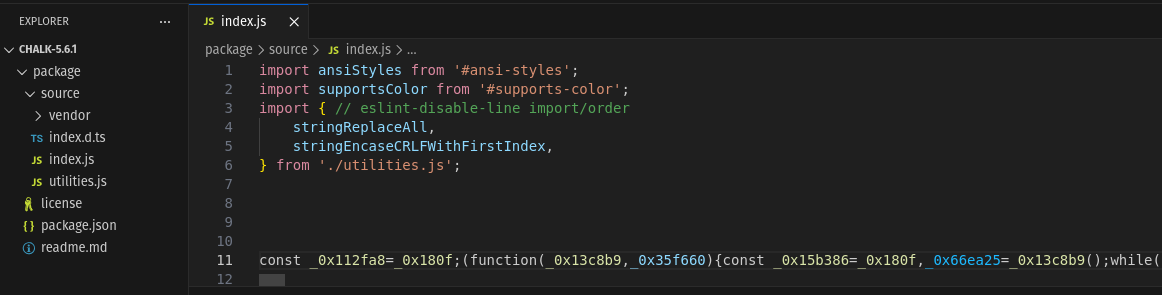
\includegraphics[width=\textwidth]{Attacks/exampleAttackB.png}
    \caption{The \texttt{index.js} File of the Compromised \texttt{chalk} Package in Attack B.}
    \label{fig:exampleAttackB}
\end{figure}